\section{Approach} \label{approach}
    In this chapter we will have a closer look on the different components of our approach. In figure \ref{fig:pipeline} you can see an overview of our approach. As mentionend in chapter \ref{intro} our approach consists of four components. In figure \ref{fig:pipeline} there are five components, this is due to the fact that we implemented an evaluator component to evaluate our results during development. For evaluation we used the topics and the corpus from previous years of Touché (2021 and 2020).

    \begin{figure}[h]
        \centering
        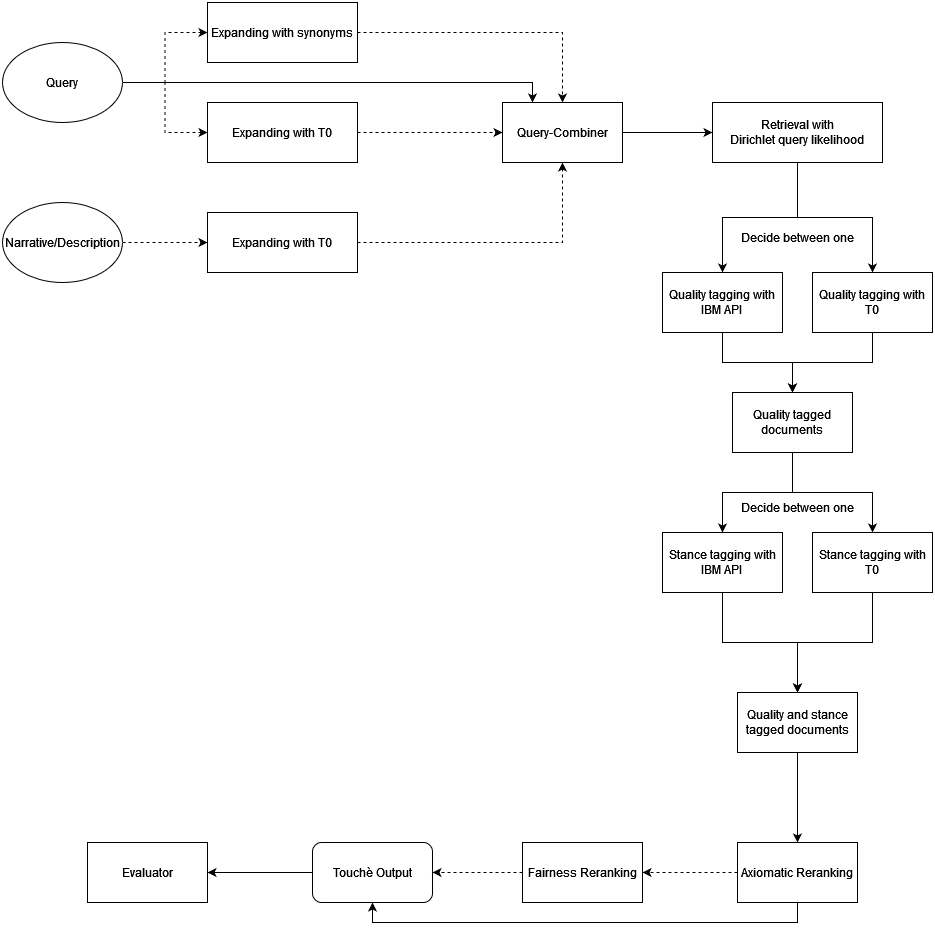
\includegraphics[scale=0.4]{figures/pipeline}
        \caption{Architecture Overview}
        \label{fig:pipeline}
    \end{figure}

    \subsection{Query Reformulation and Query Combiner}
    \subsection{Retrieval of passages}
    \subsection{Argument quality and stance tagging}
    \subsection{Axiomatic Reranker}